
%images used:
\pgfdeclareimage[width=0.45\textwidth]{gui-final}{pictures/gui_final1.png}
\pgfdeclareimage[width=0.45\textwidth]{gui-input-csv}{pictures/define-inputs-csv.png}
\pgfdeclareimage[width=0.45\textwidth]{gui-input-editor}{pictures/define-inputs-editor.png}
%~ \pgfdeclareimage[width=0.45\textwidth]{gui-final}{pictures/gui_final_spitscreen.png}

\newcommand{\screenshotScale}{1.4}



\section{Description of Zelula}
Zelula is a modelling and simulation package which enables users to simulate the protein \textit{logic} in a cell. With a provided set of BioBricks representing the basic AND and NOT gates, the user is able to design more complex circuits of interactions between the different BioBricks. The resulting circuits can be simulated and the results will be presented as a concentration/time graph.


\subsection{Circuit editor}
\begin{figure}[h!]
\centering\begin{tikzpicture}[scale=\screenshotScale]
        \pgftext[left, base]{\pgfuseimage{gui-final}}
        \draw [draw=red,very thick] (0, 2.4) -- (0, 3.7) -- (7.15, 3.7) -- (7.15,0.14) -- (1.5,0.14) -- (1.5, 2.4) -- (0,2.4);
\end{tikzpicture}
\end{figure}

\noindent Zelula enables the user to intuitively construct circuits from the basic available building blocks. Gates can be dragged from the sidebar to arbitrary positions in the working area. Connections between the gates can easily be dragged from and to the \textit{input} and \textit{output} connectors and the endpoints on gates. 

When a connection is made, no protein is selected for it by default. The user may select which protein to use. Visual feedback on protein assignment is provided through the colors of the connections.

The interface prevents the user to make some simple mistakes. For example, it's impossible to connect two inputs. If the user connects one output to two inputs, the interface makes sure the protein on those connections is the same.

Even the position of the circuits' input and output connectors can be freely chosen by dragging them using the text as an handle.

Removing gates and connection is a matter of double clicking on them.

\subsection{Compound library}
\begin{figure}[h!]
\centering\begin{tikzpicture}[scale=\screenshotScale]
        \pgftext[left, base]{\pgfuseimage{gui-final}}
        \draw [draw=red,very thick] (0,0.14) rectangle (1.5, 2.5);
\end{tikzpicture}
\end{figure}

\noindent Every circuit can be saved as a compound gate, which means it can easily be reused in later circuits. The saved compound gates are presented to the user in the sidebar, below of the basic gates. When a user drags a compound gate to the working area, it will expand to the original arrangement of gates, with the inner connections in place. The only thing left for the user is connecting it to the rest of its circuit.

\subsection{Validation}
When a user is satisfied with his work, he can validate the circuit. Different errors like unassigned proteins or inclomplete connections will be reported. The user will see the error message below the circuit, providing excellent overview to both the circuit and the errors to solve the problem.

\subsection{Simulation}
A valid circuit can be simulated. In order to simulate a circuit, the input must be defined as a function of time. Zelula provides two ways to accomplish this. Firstly, in an input editor the level for each input can be defined as a function of time in a visual way, secondly, a CSV text can be provided describing the transitions as a function of time.

\paragraph{Input editor}
\begin{figure}[h!]
\centering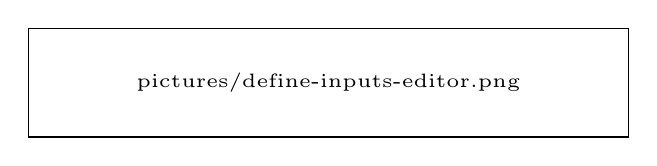
\begin{tikzpicture}[scale=\screenshotScale]
        \pgftext[left, base]{\pgfuseimage{gui-input-editor}}
\end{tikzpicture}
\end{figure}

\noindent The input editor enables the user to define each input signal in a visual way. Each tick represents a number of seconds in the simulation. The user can select this number of seconds, and also the number of ticks available.

When a user clicks on a tick, it is toggled. The user may also select ranges by clicking on a certain tick an dragging the mouse to another tick while holding the mouse button.

\paragraph{CSV input}
\begin{figure}[h!]
\centering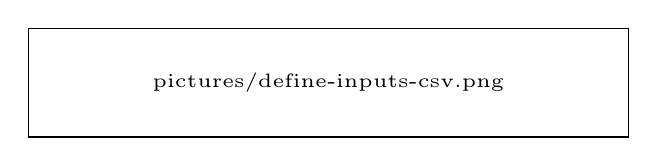
\begin{tikzpicture}[scale=\screenshotScale]
        \pgftext[left, base]{\pgfuseimage{gui-input-csv}}
\end{tikzpicture}
\end{figure}

\noindent The input may also be defined by a simple CSV format, as defined by the SA.

\subsection{Exporting}
The work done in Zelula can be shared in two different ways: the user can export the circuit to a SBML file, a common format uses in synthetic biology.

Secondly, the the graph that visualizes thee simulation output can be exported to a number of different image formats.

Of course if the user has access to the server like when it is ran locally, the user can simply save the circuit using the editor to obtain it in our application specific format (\verb=.syn=) that contains all information that was present in the application.

\subsection{Server}
The server operates in the background, serving the files and data needed for the GUI, providing persistent data storage and simulation services. The user does not interact with it in a direct way, and no server is required to be present for modelling and design. Each service of the server is provided by a Java servlet. These servlets depend on the Apache Tomcat webserver and might be distributed as a \verb|.war| archive. 
